%Asynchronous AGREE AADL Execution and Scheduling Model
%A system consists of a set of threads, a schedule, and a set of AGREE contracts.

We define a signal $x$ as a sequence of values $(x_1, x_2, ...)$ of a certain data type. That is, $x = N \mapsto T$, where $x_i$ is of type $T$ for all $i \in N$. The data type can be either a primitive data type (e.g. real, bool, int, and enumeration types) or a composite data type (e.g. record types). Assume the data type of signal $x$ and $y$ is $X$ and $Y$, respectively, $x = y$ means that $X=Y$ and $x_i = y_i$ for all $i \in N$. 

The ports of an AADL thread are modelled as signals. In particular, an event port is modelled as a sequence of Boolean values. The value \emph{true} or \emph{false} represents the event is \emph{present} or \emph{absent}, respectively. An event data port is modelled as a pair of signals, one representing the data stream, and the other representing the associated event stream. To simplify the notation, we use the port name $p$ to denote its associated data signal, and $e(p)$ to denote its associated event signal. The ports of a thread are divided into two sets: input ports (I) and output ports (O). Correspondingly, the associated signals are divided int to input signals and output signals. A thread is modelled as a collection of input signals and output signals.
%A thread could be aossciated with /emph{local} states, which are not accessible outside the scope of the thread. They are modelled as signals, noted as set S . 
A \emph{connection} between an input port $i$ and an output port $o$ establishes the equality of their associated signals $i = o$ and $e(i) = e(o)$. For simplicity, we define $e(p) = false^*$ if $p$ is a data port.

{\bf virtual events.}
We introduce two virtual input event ports: \emph{dispatch} ($d$) and \emph{complete} ($c$) for each thread.  The \emph{Dispatch} and \emph{Complete} event models, respectively, the begining and end of the time slot that a scheduler allocated to a thread to run. We assume a thread always completes its execution within the time slot. In other words, there is no pre-emption. 

{\bf thread execution.}
A thread execution starts after the arrival of its \emph{dispatch} event. This is also when the input values are frozen. This means the input values sampled for execution will not change even if new input values arrives after \emph{dispatch}. For an input event data port, its value is considered only when its event is present at \emph{dispatch}. The input read is non-blocking. In other words, a thread will not halt its execution due to waiting for an input data.
A thread's ouput signal ($o$) value can be updated only when its \emph{complete} event port ($c$) evaluates to \emph{true}, otherwise it holds its previous value. That is, if $e(c_i)=false$ then $o_i = o_{i-1}$  and $e(o_i) = e(o_{i-1})$ for all $i \in N$ and $o \in O$. We denote the initial value of a signal as $x_0$. For an event port $p$, $e(p_0) = false$. The output write is also non-blocking. In other words, a thread will not halt its execution due to waiting for an previous output data to be \emph{consumed}. It simply overwrites.

{\bf schedule.}
A schedule of a set of threads defines the \emph{dispatch} and \emph{complete} event flows of each thread. A valid schedule...

{\bf model of time.}
All signals by definition are associated with the same logic clock, indicated by its index. The \emph{tick} models the basic time unit where the system is analyzed. This could be the basic time unit used in an AADL schedule, or the greatest common divisor. For example, a schedule with period = 10 ms, thread A = 4 ms, idle = 2 ms, thread B = 2 ms,  idle = 2 ms. Then the \emph{tick} could be used model 2 ms. Then, d(A)=(1,0,0,0,0)*, c(A) = (0,0,1,0,0)*, d(B) = (0,0,0,1,0)*, c(B) = (0,0,0,0,1)*.

{\bf model of execution delay.}
The thread exeution delay is not directly modelled. Instead, the time slot allocated to a thread in a schedule is modelled by the \emph{distance} between the thread \emph{dispatch} and \emph{complete}. If we assume there is no pre-emption, this modells  the worst case execution time or deadline.

%{\bf model of communication delay.}
%The communication delay is abstracted out. However, in a schedule there is often a time window between the complete event of the one thread and the dispatch event of the next thread. This time window models the %worst case communication delay.

{\bf AGREE contracts.}

Our approach to modelling the AADL asynchronous MoC in AGREE is to keep the existing AADL model structure intact and add new AGREE contracts and modify existing contracts. The added contracts model the asynchronous communication between AADL ports. The modification of the exisiting contracts reflcts the interpretation of the contracts (system properties) under the asychronous MoC. 


\begin{figure}[ht!]
\centering
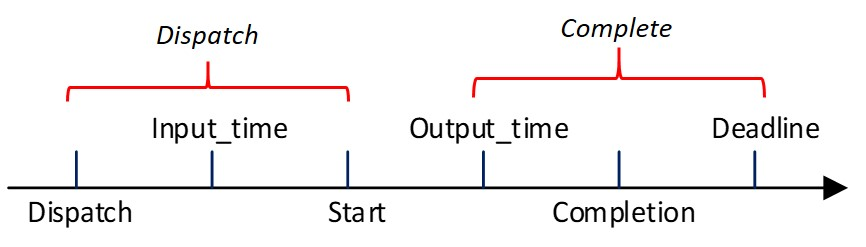
\includegraphics[width=80mm]{aadl_events.jpg}
\caption{An AADL Model with AGREE Contracts\label{motivation}}
\end{figure}

In asynchronous AGREE, the \emph{Execution\_Time} property is modelled by the time interval between the \emph{Dispatch} event and the \emph{Complete} event.
The assumptions hold at the \emph{Dispatch} event \[Dispatch => Assumption\] , and the guarantees hold at the \emph{Complete} event, i.e. \[Complete => Guarantee\] 

% Assumptions
We make the following assumptions. The \emph{Input\_Time} property value is unspecified, thus default to dispatch time. The \emph{Output\_Time} property value is unspecified, thus default to the execution completion time. The \emph{Queue\_Size} property value is unspecified, thus default to size one. The \emph{Execution\_Time} property represent a single value, not a real range. The \emph{Dispatch\_Protocol} property value is periodic. The \emph{Timing} property value of each connection is unspecified, thus default to immediate connection. There is no simultaneous read and write access to a queue or buffer (data port). If an event data queue or a data port buffer is empty, the most recent data is used. The \emph{Dequeue} occurs at every dispatch. There is no preemption. There is no propagation delay.

% Modelling
For an output event data port of a thread, the event and data holds till the thread's next \emph{Complete} event. This is represented by the following AGREE contracts.

\begin{math} 
not Complete => (event(Port) = prev(event(Port), false))
\end{math} 

\begin{math}
not Complete => (true -> (Port = pre(Port)))
\end{math}  

% Rational
The output event hold models the latching behavior of an event queue (size one). At the end of execution of a thread, an output event may or may not be raised. However, the AGREE contracts representing the functional requirements only ensures an event is raised only at that exact time instant (i.e. \emph{Complete}). The event is latched so that the target thread, once dispatched, samples the correct result. The consideration for the output data hold is similar.
 
% Schedule
In asynchronous AGREE, a schedule defines the sequential execution order of threads. It is specified by the user. It often come from the actual software execution schedule on the target platform (e.g. seL4 domain schedule). Currently AADL does not define a standard format to specify a schedule. We used AGREE \emph{assumption} on each thread's \emph{Dispatch} and \emph{Complete} event to represent a schedule. For example, \emph{assume "schedule" :			ThreadA\_Dispatch = (Frame = 60) and ThreadA\_Complete = (Frame = 70) and ...}